\documentclass[onecolumn]{IEEEtran}
\usepackage{graphicx} % Required for inserting images
\usepackage[spanish]{babel}
\usepackage{amsmath}
\usepackage{xfrac}

\title{Introducción a Inteligencia Artificial\\Detección de SPAM}
\author{Gonzalo Gabriel Fernández (e1911)}
\author{\IEEEauthorblockN{Gonzalo Gabriel Fernandez\IEEEauthorrefmark{1},
Roberto Enrique Castro Beltran\IEEEauthorrefmark{2}}\\
\IEEEauthorblockA{Carrera de Especialización en Inteligencia Artificial\\
Universidad de Buenos Aires\\
Email: \IEEEauthorrefmark{1}fernandez.gfg@gmail.com,
\IEEEauthorrefmark{2}electrobot73@gmail.com}}
\date{\today}

\begin{document}

\maketitle

\begin{abstract}
Uno de los problemas más comunes en la clasificación es la detección de correos electrónicos SPAM. Uno de los primeros modelos utilizados para abordar este problema fue el clasificador de Bayes ingenuo. La detección de SPAM es un problema persistente en el mundo digital, ya que los spammers continúan adaptando sus estrategias para eludir los filtros de correo no deseado. Además del clasificador de Bayes ingenuo, se han desarrollado y utilizado una variedad de técnicas más avanzadas en la detección de SPAM, que incluyen algoritmos de aprendizaje automático, redes neuronales y métodos basados en reglas.
\end{abstract}

\section{Descripción del problema}
En este trabajo práctico, utilizaremos un conjunto de datos que consta de 4601 observaciones de correos electrónicos, de los cuales 2788 son correos legítimos y 1813 son correos SPAM. Dado que el contenido de los correos electrónicos es un tipo de dato no estructurado, es necesario procesarlo de alguna manera. Para este conjunto de datos, ya se ha aplicado un procesamiento típico en el Procesamiento del Lenguaje Natural (NLP), que consiste en contar la frecuencia de palabras observadas en los correos.

El procesamiento de lenguaje natural (NLP) desempeña un papel fundamental en la detección de SPAM, ya que permite analizar el contenido de los correos electrónicos y extraer características relevantes para la clasificación. Además de contar la frecuencia de palabras, se pueden utilizar técnicas más sofisticadas, como la extracción de características semánticas y el análisis de sentimientos, para mejorar la precisión de los modelos de detección de SPAM.

En este proceso, se cuenta la cantidad de ocurrencias de cada palabra en los diferentes correos.

Con el fin de preservar la privacidad de los mensajes, la frecuencia de palabras se encuentra normalizada. El conjunto de datos está compuesto por 54 columnas de atributos que se denominan:

word\_freq\_XXXX: Donde XXXX es la palabra o símbolo. Los valores son enteros que van de 0 a 20k.
Además, hay una columna adicional llamada spam, que es 1 si el correo es SPAM o 0 si no lo es.

Los clasificadores de Bayes ingenuos fueron los primeros filtros utilizados por las aplicaciones de correo electrónico, basados en este principio de palabras. La idea es que, partiendo de un dato a priori sobre la probabilidad de que un correo sea SPAM o no, ciertas palabras nos indicarán que la probabilidad a posteriori, dadas esas palabras, es más probable que el correo sea SPAM o no.

Para este trabajo práctico, se proporciona una notebook (ayuda.ipynb) con la lectura del conjunto de datos, la separación de los datos, entre otras ayudas para resolverlo.

\newpage
\section*{Análisis del conjunto de datos}
Las 10 palabras más encontradas en correos SPAM son:
\begin{itemize}
    \item 'you'
    \item 'your'
    \item 'will'
    \item 'free'
    \item 'our'
    \item '!'
    \item 'all'
    \item 'mail'
    \item 'email'
    \item 'business'
\end{itemize}

Las 10 palabras más encontradas en correos no SPAM son:
\begin{itemize}
    \item 'you'
    \item 'george'
    \item 'hp'
    \item 'will'
    \item 'your'
    \item 'hpl'
    \item 're'
    \item 'edu'
    \item 'address'
    \item 'meeting'
\end{itemize}

Las palabras en común son: 'you', 'will' y 'your'.

\section*{Clasificador de Bayes ingenuo y de regresión logística}
Del conjunto total de datos se obtuvo un conjunto de entrenamiento y un conjunto de prueba (70\% y 30\% respectivamente).

Para clasificar los datos se utilizaron dos modelos: un clasificador de Bayes ingenuo y uno de regresión logística. Para ambos se utilizó la biblioteca \textit{scikit learn}.

Se entrenó ambos modelos con el conjunto de datos para entrenamiento.

\section*{Análisis de tipo de error}

En la figura \ref{fig:confussion-matrix} se puede observar las matrices de confusión para los dos clasificadores utilizados.

\begin{figure}[ht]
    \centering
    \includegraphics[width=0.9\linewidth]{confussion_matrix.png}
    \caption{Matriz de confusión para modelos entrenados}
    \label{fig:confussion-matrix}
\end{figure}

De la figura \ref{fig:confussion-matrix} se observa que:
\begin{itemize}
    \item El clasificador de Bayes ingenuo comete más errores de tipo I (falso positivo).
    \item El clasificador de regresión logística comete una ligera mayor cantidad de errores de tipo I.
\end{itemize}

Errores de tipo I y tipo II en detección de Spam:

\begin{itemize}
    \item Error de tipo I (falso positivo):
    \begin{itemize}
        \item Un correo legítimo es clasificado como spam.
        \item Consecuencia: El usuario podría perder correos importantes que fueron enviados a la carpeta de spam.
    \end{itemize}
    \item Error de tipo II (falso negativo):
    \begin{itemize}
        \item Un correo spam es clasificado como legítimo.
        \item Consecuencia: El usuario recibe correos no deseados en su bandeja de entrada, lo que puede ser molesto y potencialmente peligroso si contiene phishing o malware.
    \end{itemize}
\end{itemize}

Para el problema de detección de spam, los errores de tipo I (falsos positivos) son más importantes porque implican la pérdida de correos legítimos, lo cual puede tener consecuencias significativas para el usuario.

\section*{Resultados obtenidos}

En la tabla \ref{tab:performance-metrics} se observa la precisión y la recuperación obtenida para cada clasificador utilizado.

\begin{table}[ht]
\centering
\begin{tabular}{|l|l|l|}
\hline
 & Precisión & Recuperación \\ \hline
Clasificador de Bayes ingenuo & 0.77 & 0.96 \\ \hline
Clasificador de regresión logística & 0.86 & 0.88 \\ \hline
\end{tabular}
\caption{Resultados de precisión y recuperación para los modelos utilizados.}
\label{tab:performance-metrics}
\end{table}

Las métricas evalúan lo siguiente:
\begin{itemize}
    \item La precisión mide la proporción de verdaderos positivos sobre el total de predicciones positivas. Una alta precisión significa pocos falsos positivos.
    \item La recuperación mide la proporción de verdaderos positivos sobre el total de verdaderos positivos y falsos negativos. Una alta recuperación significa pocos falsos negativos.
\end{itemize}

Ambos modelos presentaron errores de tipo I (falsos positivos) en mayor proporción, sin embargo, el clasificador de Bayes ingenuo tuvo un mayor numero de errores de este tipo, es por ello que su precisión es menor comparado con la regresión logística.

\section*{Curva ROC}

En la figura \ref{fig:roc} se  observa la curva ROC y el AUC (Área Bajo la Curva ROC) de ambos clasificadores.

\begin{figure}[ht]
    \centering
    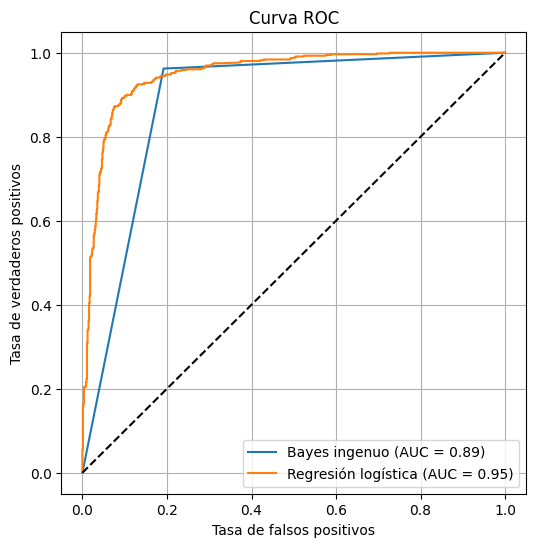
\includegraphics[width=0.5\linewidth]{roc.png}
    \caption{Curva ROC y AUC para los modelos utilizados.}
    \label{fig:roc}
\end{figure}

\end{document}
